\documentclass[12pt,a4paper]{report}
\usepackage[utf8]{inputenc}
\usepackage[francais]{babel}
\usepackage[T1]{fontenc}
\usepackage{amsmath}
\usepackage{amsfonts}
\usepackage{amssymb}
\usepackage{graphicx}
\graphicspath{{pic/}}
\usepackage{authblk}
\author{Renan Husson, Quentin Rouland, Jerome Morjon, Matthieu Penchenat, Alexandre Pereira, Sébastien Bouyt}
\affil{Université Toulouse, Jean Jaurès - L3 MIASHS \\ Document D1 : Specification Fonctionnelle}
\begin{document}
\title{Projet Web - AJAX}
\maketitle
\renewcommand{\contentsname}{Sommaire}
\tableofcontents
\chapter*{Introduction}
\addcontentsline{toc}{chapter}{Introduction}
Séance 1 26/01/2015 : \\
Animateur : Renan Husson
Secrétaire : Matthieu Penchenat
\newline

Séance 2 27/01/2015 : \\
Animateur : Matthieu Penchenat
Secrétaire : Quentin Rouland
\newline

Objectif :
Comprendre le sujet
Préparer un document de spécification
Préparer les questions clients
Proposer des idées innovantes pour le projet
\chapter{Spécification}
\section{Speech}
Dans le cadre du programme culturel de la mairie de Toulouse, les enfants des écoles maternelles effectuent en 2015 une visite au musée des Augustins. Afin de préparer cette visite, il serait intéressant de proposer des outils numériques visant à introduire de manière ludique et interactive le musée et ses œuvres auprès des enfants.\\
La Mairie de Toulouse nous a donc demandé de réutiliser des données ouvertes publiés sur son portail dans l'objectif de créer un application web visant un public de 4 à 5 ans accompagné de leur adulte référent. La finalité de l'ensemble de l'application devra être la découverte de la culture par les enfants de maternelle.
Pour ce projet, nous allons devoir réaliser un site responsive qui puisse être adapté sur smartphone, tablette ainsi que sur ordinateur. Ensuite, il faut que ce site soit ergonomique et facile d'utilisation pour un enfant. Il faut qu'il soit intuitif et simple d'utilisation ainsi qu'éducatif et culturel.
- Jeux
- Description adulte référent
- Finalité de l'application
\section{Use Case}
\begin{figure}[!h]
\centering
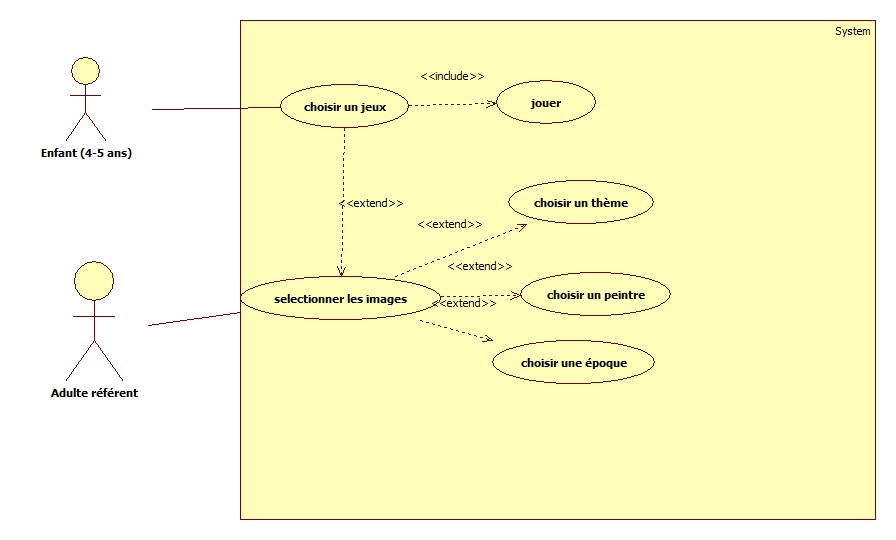
\includegraphics[width=350px]{uml.jpg}
\end{figure}
\subsection{Acteurs}
Enfants et adultes référents
\chapter{Questions à poser au client}
\begin{itemize}
\item C'est qui cet adulte référent? Plusieurs?
\item Il choisi des images pour tout le monde?
\item Admin, acteur?
\item Si c'est côté client ou côté administrateur?
\item Niveau des enfants 4, 5 ans? (les enfants ne savent pas lire)
\item De quoi disposons comme information?
\item Referent est il toujours present lorsque l'enfant joue?
\item Referent a un jeux ou plusieurs atcifs simultanement?
\end{itemize}
\chapter{Idées}
Liste de jeux ;
\begin{itemize}
\item Jeux 94 (avec images?)
\item Jeux du pendu
\item Mélange pour facilité (de jeux)
\item Mémo et puzzle (compulsory)
\end{itemize}

\medbreak
Technologies :
\begin{itemize}
\item Utilisation d'un "text to speech" : API Goolgle
\item Utilisation d'un "speech to text" : pas d'API correcte trouvée
\item Base SQL : MySql
\item Utilisation d'un Framework PHP MVC : .codeigniter
\item Utilisation Framework CSS : Bootstrap
\end{itemize}

\medbreak
Fonctionnement global (prévison) :
\\Page d'accueil : on retrouve les images de profile des référents ayant une session actives de jeux.
L'enfant clique sur sur l'image de son référent et arrive dans le jeux sélectionné par celui-ci.
Le référant peut se connecter afin de créer des sessions de jeux et les activer, les supprimer.
%\listoffigures
%\addcontentsline{toc}{chapter}{Table des illustrations}
%\renewcommand{\bibname}{Références}
%\begin{thebibliography}{9}
%\bibitem{lamport94}
% Arte Reportage (arte futur).
%Disponible sur http://www.arte.tv/guide/fr/plus7/,
%2014.
%\end{thebibliography}
%\addcontentsline{toc}{chapter}{Références}
\end{document}
